\subsection{Iteration \#4}

Data analysis is done first by a general overview in Google Sheets, by statistical analysis in R, and by a parallel coordinates visualization. The process to do this, is described below.

\subsubsection{Data Acquisition from Server}

It was desired to store the data in Google Sheets, thus it was necessary to collect the MongoDB database content, and convert JSON format into a Google Sheets-readable format, like CSV.

Multiple approaches were tried, and the Google Chrome extension called Magic Json by agaze\_dev\_team (last updated October 29, 2015) %https://chrome.google.com/webstore/detail/magic-json/cajifcebjiflndefndbnoeenjpiiiagm?hl=en
was the one that worked without problems. \citep{agaze}.

\subsubsection{Data Acquisition from Pre-Study}

The Pre-study data acquisition was done by instead of looking at the paper-submitted pre-study evaluation forms, using the data processed into Google Sheets.

\subsubsection{Data Enhancement of Server Results}

This section presents how data from the server was processed, to enable visualization mapping.

To make the data easier to work with, the columns were reordered, and made sortable and filterable.

Some columns were given conditional formatting, so it would be easier to spot irregularities. After this, some observations could be made.

\todo{Lägg till bild "results-colored.png" (finns på skrivbordet)}

To be able to compare the test results with the pre-test results, it was clear that it would not be viable to test every dimension against every dimension.

Instead, since goals of the app evaluation had been predefined in the following way, the quiz results were summarized into a new sheet so that the following could be derived:

\begin{itemize}
\item \% correct 1st try
\item number of tries until 100\%
\item number of tries until 100\% in 1 try
\end{itemize}

These could be calculated by having columns for:

\begin{itemize}
  \item Quiz 3
  \begin{itemize}
    \item Start time training
    \item \% correct 1st try
    \item number of tries until 100\% in 1 try
    \item Time difference start to end time certification
  \end{itemize}
  \item Quiz 9
  \begin{itemize}
    \item Start time training
    \item \% correct 1st try
    \item Time difference start to end 1st try
    \item Time difference start to passed training
    \item Time difference 1st try to certified
  \end{itemize}
\end{itemize}

Then, to see trends, I again added color scales. With ordinal values, a sequential color scheme is used (e.g. fastest time, from green to red), and with nominal values (like if they are female or male) where there is no right value, a qualitative color scheme is used. Now, it was easier to spot outliers and trends.

\subsubsection{Date Enhancement of Pre-study Results}
To see differences in answers more clearly, the data from the pre-study was made sortable and filterable. Then, the data was resampeled for each column that hade numerable (sortable) data in text instead of numbers, so e.g. "The day before" was changed to -1 and "The same day" to 0. In a similar way, school level was divided into four different groups, from 0 to 3, where 0 meant secondary, year unknown, 1 meant lower secondary, 2 meant upper secondary, and 3 meant tertiary.

After this, each column was given conditional formats using a color scale, using Google Sheets built-in functionality. This gave a visual way to quickly get a overview of the pre-test data.

\subsubsection{Data Enhancement by joining Pre-test and Results Summary}

I joined the summary sheet and the pre-quiz sheet, meaning I had created a multiple-variate data set (serveral dimensions that I needed to compare with several dimensions), see figure \ref{fig:analysFarg3}.

\begin{figure}[h]
    \centering
    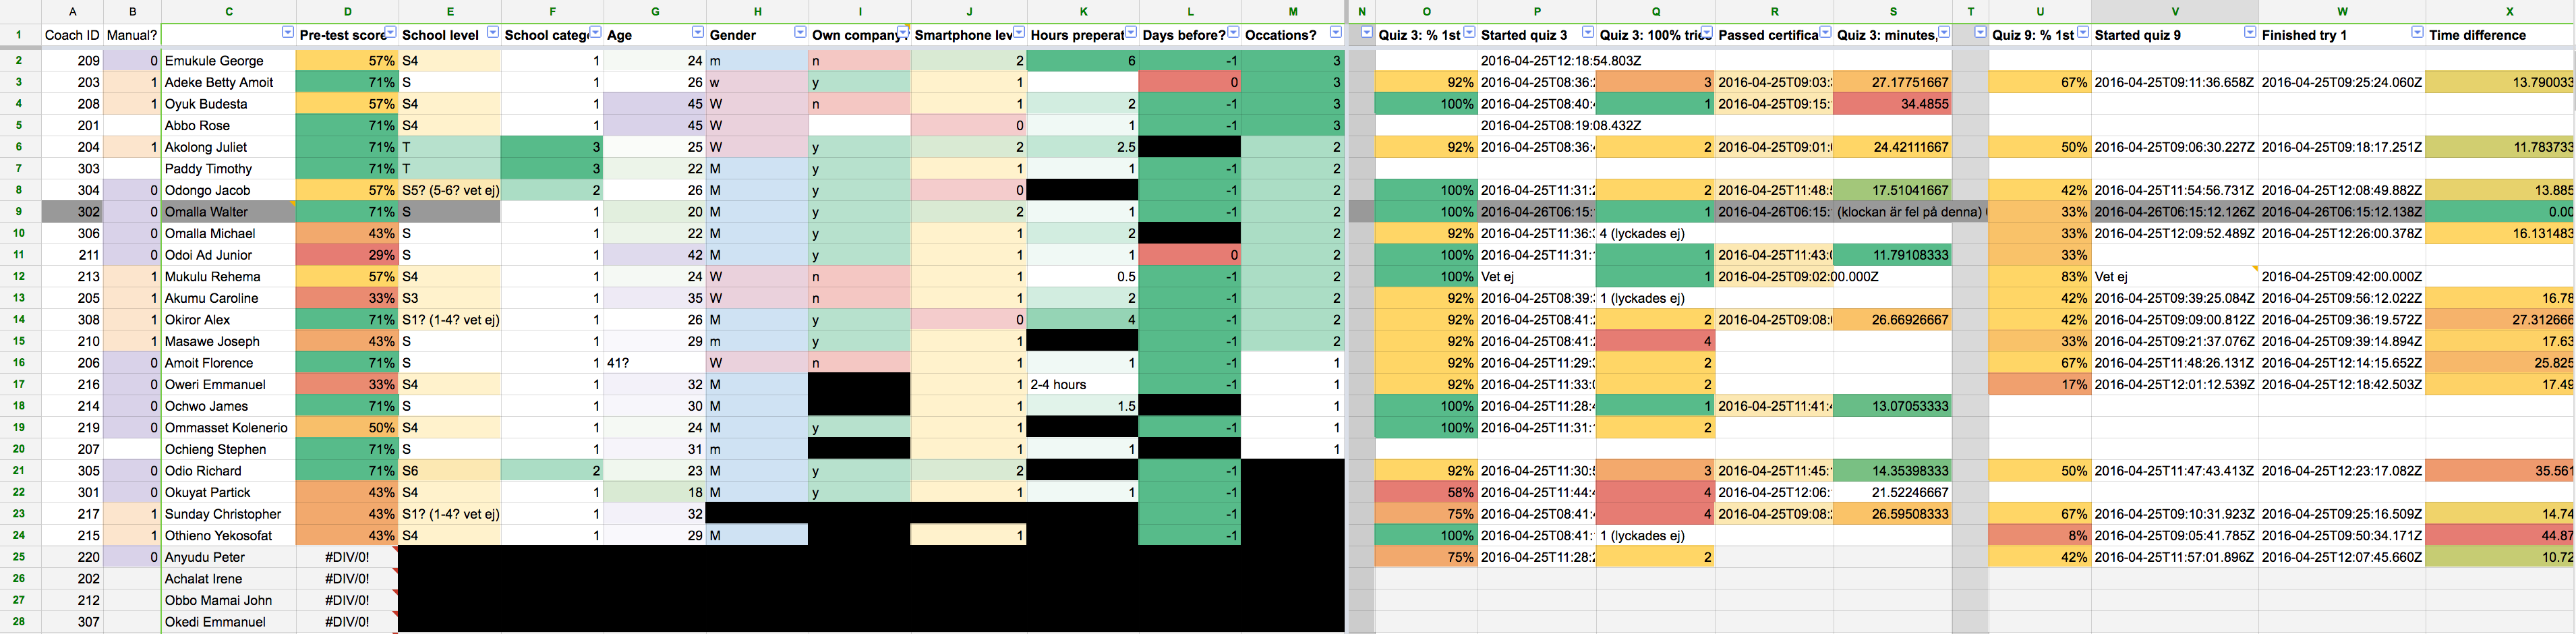
\includegraphics[width=0.7\textwidth]{analysis/analysFarg3.png}
    \caption{The mutli-variate data set, made filterable and sortable in Google Sheets. Color scales and calculating means makes it easier to compare characteristics of the coach together with pre-test and quiz results. However, it is cumbersome and hard to quickly filter data on multiple parameters.}
    \label{fig:analysFarg3}
\end{figure}

I met with my university supervisors, so they could further support me in how to properly analyze the data. Since the two control groups showd similar means on the pre-quiz results, the two control groups were determined comparable.

To meet the challenges of using Google Sheets, a multivariate analyzation software or a visualization was suggested to discover the data in less time.

It was hard to determine a suitable multivariate analysis software suitable when having so few data points. Principle Component Analysis or Cohen's kappa would not be suitable, neither was it believed applicable to do Linear correlation on all dimensions.

After discussion with other Master thesis students working with analysing data from various disciplines, parallel coordinates was suggested. It would allow me to very quickly filter the data, find correlations, and distinguish outliers and common characteristics.

To guide the usage of the parallel coordinates (as there is so much to discover in the data set), using R to do Logistic correlation was also done. A disadvantage with this method, is that to be statistically significant, many data points may be needed, and it was now known before-hand if the method would be useful. Probably, parallel coordinates would be the best method with analysing a small multi-variate data set.

\subsubsection{Visualization Mapping}
The goal with visualization mapping is to generate renderable data, in my case for the parallel coordinates visualization.

Thus, I added a new spreadsheet, specific for visualizing the data.

I deleted columns that would serve no visual purpose (e.g. timestamps), gave all cells data values (even N/A when undefined), deleting users that did not have data, and shortened the column names so they would fit on the screen.

The data was then exported from the Google Sheet into CSV.

\subsubsection{Rendering}

For rendering, the JavaScript library D3.js was chosen. It supports data-driven documents for visualizing data with HTML, SVG and CSS. It supports both JSON and CSV data.

A visual framework for multidimensional detectives for D3.js was found, called "Parcoords.js", written by Chang Kai (2012).
% https://syntagmatic.github.io/parallel-coordinates/
% Chang, K. (2012). Parallel Coordinates toolkit : Parcoords.js 0.1. Parallel Coordinates toolkit. Retrieved September 8, 2012, from http://syntagmatic.github.com/parallel-coordinates/
% Kosara, R. (2010, May 13). Parallel Coordinates. Eagereyes.org. Retrieved September 8, 2012, from http://eagereyes.org/techniques/parallel-coordinates
% Tricaud, S. (2008). Picviz: finding a needle in a haystack. Proceedings WASL, San Diego. Retrieved from http://www.usenix.org/events/wasl08/tech/full_papers/tricaud/tricaud.pdf

The example code from "Linking with a Data Table" provided the basis for the rendering. It would be a great benefit to bee able to see both a parallel coordinates visualization, and to see the same values present in the Google Sheet. %https://syntagmatic.github.io/parallel-coordinates/examples/table.html

The example CSV file was replaced with the data from exporting the Google Sheets data. Eventually, also the colors were changed, and addeed the toolkit's functionality to drag the axes titles around to reorder the dimensions, since the goal was to quickly compare and find correlations. The result is visible in \ref{fig:parallell-coordinates-1}.

\begin{figure}[h]
    \centering
    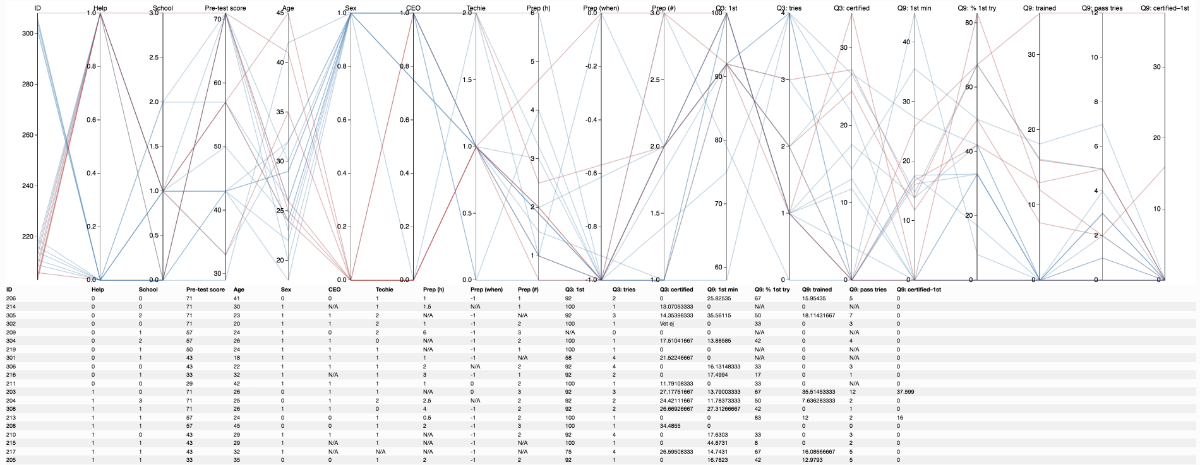
\includegraphics[width=0.7\textwidth]{analysis/parallellCoordinates1.png}
    \caption{The parallel coordinates visualization, done in d3.js. The visualization support draggable axes, filtering of data via dragging the sliders (which syncronizes with the data table), color assignment (like blue and red for men and women in the example), and hovering over a specific data point.}
    \label{fig:parallell-coordinates-1}
\end{figure}
